\documentclass{article}
\usepackage{tikz}
\title{The RAFAELIA Toroidal Quantum Processor: A Self-Verifying Continuous-Variable Architecture with Fractal Coupling}
\begin{document}\maketitle
\section{Introduction}
RAFAELIA is a continuous-variable processor on $\mathbb{T}^7=(\mathbb{R}/\mathbb{Z})^7$ with period 42 and fixed-point Q16.16 control.
\section{Mathematical Model}
State $\mathbf{s}=(u,v,\psi,\chi,\rho,\delta,\sigma)$ follows EMA $C_{t+1}=0.75C_t+0.25C_{in}$, $H_{t+1}=0.75H_t+0.25H_{in}$, and $\phi=(1-H)C$.
Forward recurrence is $F_{n+1}=F_n\frac{\sqrt{3}}{2}-\pi\sin(279^\circ)$ with period 42.
\section{Hardware Architecture}
Integrated photonics with OPO-like oscillators, 1000 active cells plus 8 integrity/control points (BitStack 1008).
\begin{center}
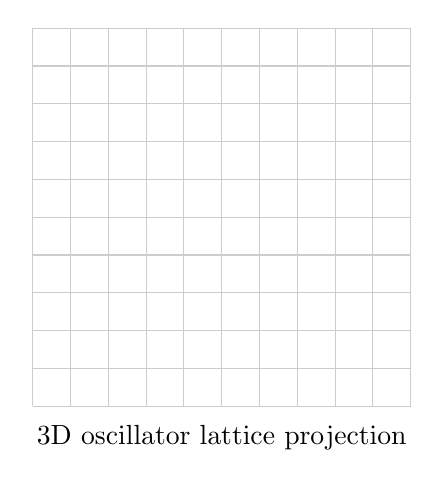
\begin{tikzpicture}[scale=0.8]
\draw[step=0.6,gray!40] (0,0) grid (6,6);
\node at (3,-0.5){3D oscillator lattice projection};
\end{tikzpicture}
\end{center}
\section{Error Correction}
Commit gate has LOAD$\to$PROCESS$\to$VERIFY$\to$COMMIT. VERIFY failure triggers rollback to optical delay-line snapshot.
\begin{center}
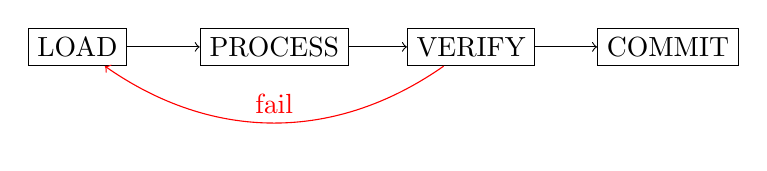
\begin{tikzpicture}
\node[draw] (l) at (0,0){LOAD}; \node[draw] (p) at (2.5,0){PROCESS};
\node[draw] (v) at (5,0){VERIFY}; \node[draw] (c) at (7.5,0){COMMIT};
\draw[->] (l)--(p);\draw[->](p)--(v);\draw[->](v)--(c);\draw[->,red](v) to[bend left=35] node[above]{fail} (l);
\end{tikzpicture}
\end{center}
\section{Programming Model}
BitRAF 42-bit instruction configures frequencies, weights, phases, partial CRC, vCPU load, and commit state each cycle.
\section{Isosceles Scheduler}
\begin{center}
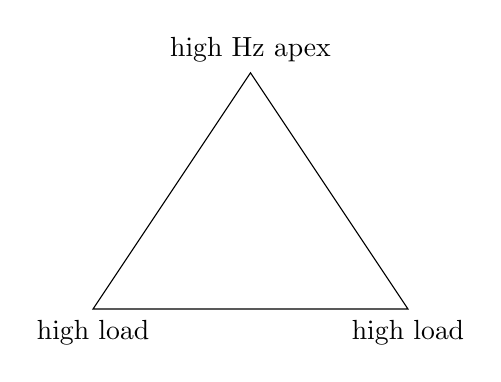
\begin{tikzpicture}
\draw (0,0)--(4,0)--(2,3)--cycle;
\node at (2,3.3){high Hz apex};\node at (0,-0.3){high load};\node at (4,-0.3){high load};
\end{tikzpicture}
\end{center}
\section{Comparison}
Compared to gate-model and annealers (e.g., D-Wave), RAFAELIA adds intrinsic cycle-level self-verification and continuous toroidal routing.
\section{Performance Estimates}
With 100 MHz control and 42-cycle canonical epochs, verification points occur every 70 ns (each 7 cycles).
\end{document}
